\section{Approach}

\cite{Difallah:2012ty}

[MAKE POINT ABOUT ONE OF THE ORIGINAL INTUITION POINTS BEING REDUCING THE ORIGINAL PROBLEM TO AN IMAGE LABELLING PROBLEM, IT'S NOT NECESSARILY OBVIOUS]
[USE \cite{Quinn:2011dj} FOR THE DEFINITION OF THE AGGREGATION PROBLEM]
[HIGHLIGHT HOW, DIFFERENTLY THAN MOST OF CROWDSOURCING IMAGE LABELLING USE CASES, HERE WE'RE COLLECTING TWO LABELS PER "SUBJECT", AND THEY'RE PRACTICALLY INDEPENDENT]
[HIGHLIGHT HOW THE SET OF POSSIBLE VALUES FOR THE LABELS IS NOT LIMITED, IT'S MORE LIKE AN NxN SPACE, N BEING THE SET OF NATURAL NUMBERS, WHERE THE FIRST N REPRESENTS THE ACTUAL NUMBERS 1, 2, 3... AND THE SECOND N THE LETTERS IN THE POSTFIX 1 -> A, 2 -> B, ..., 27 -> AA ...]

\subsection{The social machine mix}

    Although the OLAF data is conceptually simple, assembling such a large dataset as OLAF while assuring sufficient quality still is a complex task.
    
    It is our hypothesis that, to make the best use of pre-existing open data and potentially available technology and human resources, such a problem must be decomposed in a series of complementary sub-problems, each developing parts of its scope and leveraging the peculiarity of its specifications. Each problem, then, can be solved by designing a dedicated socio-technical system, or social machine. This decomposition can take place over several iterations, hence creating a hierarchy of systems that we will call the "social machine mix". 
    
    [THERE SHOULD BE AN IMAGE HERE BUT IMAGE POSITIONING IN LATEX IS TRICKY]

    \begin{figure*}
    	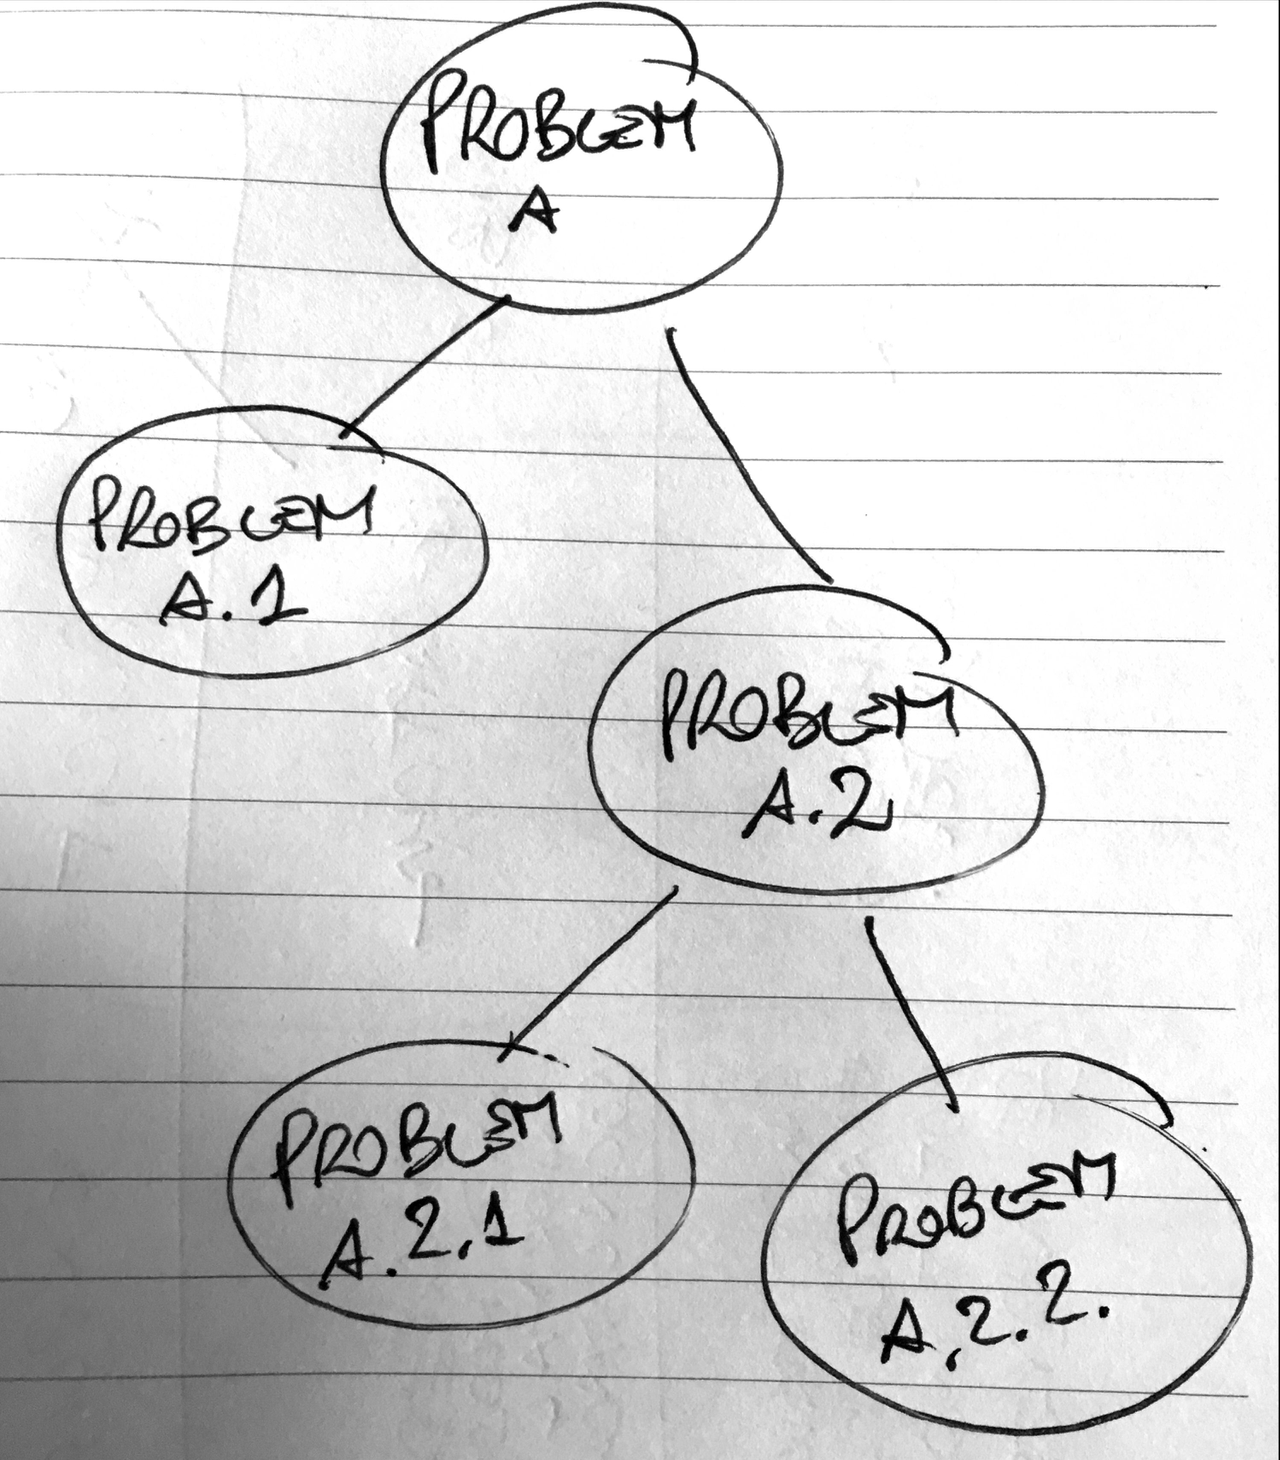
\includegraphics[width=0.95\textwidth]{social-machine-mix-1.png}
    	\caption{This picture should not be here, but apparently it is a nightmare in LaTeX.}
    	\label{fig:social_machine_mix_1}
    \end{figure*}
    
    \textbf{The central role of pre-existing open data.} 
    
    [THIS IS AN INTERESTING STATEMENT, I WONDER IF IT CAN BE GENERALISED] The main driver determining the possible decompositions of the original problem into a hierarchy of sub-problems is the availability of pre-existing and reliable open data. There are two reasons for that.

    \begin{itemize}

        \item The first and more intuitive reason is an assumption: no social machine can produce data in a more effective way than re-using a pre-published, reliable dataset is.  
        
        Hence, re-using existing open data will always be prioritised in respect to re-creating the same, e.g. using crowdsourcing. The focus of social machines in the overall mix should rather be on: a) on creating original data where the same cannot be sourced or computed, and b) on leveraging those skills where humans outperform machines. 
        
        The obvious example of this is using human contributors to survey the streets, being this in person in the physical world, or by examining pictures of the locations, that is how crowdsourcing is used in the system described later in this paper.

        \item The second reason is that open data can be instrumental to operate a social machine. Even when a dataset is not re-used directly to creating the target output data, it can be used for other functions, e.g. supporting the process by which humans contribute. There will be a clear example of this later in this paper. 

    \end{itemize}

\subsection{Scope restrictions}
    
    To make the problem suitable to research it was simplified as described below. 
    
    \textbf{Open data availability.} Although the overarching objective for OLAF is to achieve UK coverage, the availability of open data differs substantially from one UK country to another. Our approach was based on what is available for England and Wales only, as the two have the richer and most homogeneous open data offering, and their territory is estimated to include the 84\% of the 35m addresses in the UK\footnote{[FOOTNOTE EXPLAINING THE ESTIMATE, LIKELY TO BE MADE USING NO. OF HOUSEHOLDS BY COUNTRY FROM ONS AS AN INDICATION OF NO. OF BUILDINGS HENCE ADDRESSES]}.
    
    The validity of the approach is independent of the geographical region that is the subject of the study, as long is the problem is consistent, e.g. the definition of the address is the same. The moment the same open data used for England and Wales becomes available for Scotland and Northern Ireland, the method can be deployed to produce an UK-wide OLAF without modification. Alternatively, if that would not happen, complementary social machines would need being added to the mix.
    
    \textbf{Sample territory.} Within the territory described above, the experiments were performed to address just a sample of the London area, made of five tiles [MORE TECH DESCRIPTION OF WHAT THEY ARE]. This is the same sample that was used in literature in the past to analyse the performance of other geospatial data crowdsourcing initiatives, e.g. OpenStreetMap in [REFERENCE].
    
    \begin{figure*}
    	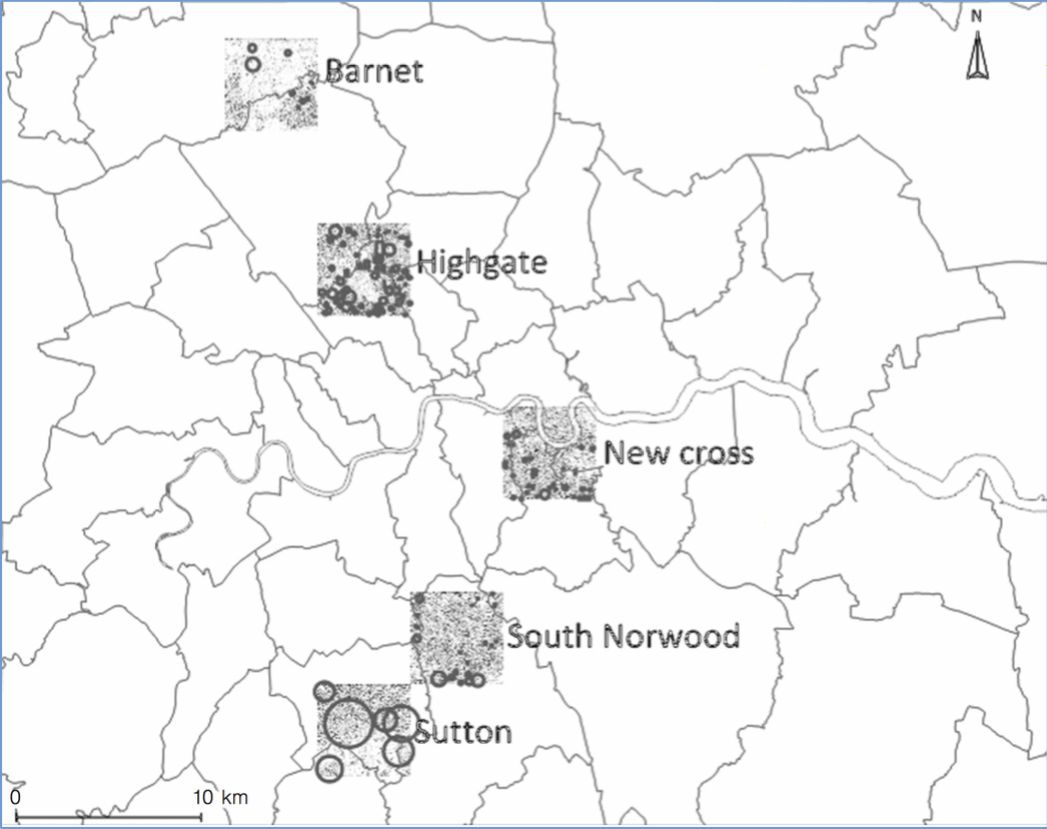
\includegraphics[width=0.95\textwidth]{london-sample-1.png}
    	\caption{This picture should not be here, but apparently it is a nightmare in LaTeX.}
    	\label{fig:london_sample_1}
    \end{figure*}
    
    More precisely, a road is considered in scope if its bounding box, as defined by Ordnance Survey's "Open Names", is completely included in any of the five tiles. 
    
    [SOME WORDING FROM THAT PAPER TO STATE HOW WE DID NOT SIMPLIFY THE PROBLEM BY DOING THIS BUT JUST REDUCED IT IN SIZE].
     
    \textbf{Named vs numbered roads.} Roads that are identified by a number only, e.g. as for motorways, will be considered out of scope.
    
    \textbf{Reliability of the sources.} Only open data from authoritative sources was considered as an option in defining the approach, such as government bodies', and it is assumed to be of the highest possible quality, equivalent to what could be called {\it ground truth}. This allowed the approach not to include any validation of the sources.

